\documentclass{report}
\usepackage[backend=biber]{biblatex}
\usepackage{pdfpages} 
\usepackage{hyperref}


\bibliography{abgabe}
\graphicspath{{images/}}

\begin{document}	
	\tableofcontents
	\chapter{First ever lateX chapter}
	\section{Well, this is a section}
	Will this work as intended?
	$$ a^2 + b^2 = c^2$$
	\subsubsection{It sure did}
	This too?
	\section{Formel 1}
	Kimi Antonelli has currently the most points \cite[S. 1]{Formel1}.
	\chapter{If that isn't a second chapter}
	\section{A image}
	This should be a cat (siehe Abb.~\ref{fig:Cat}).
	\begin{figure}
	\centering
	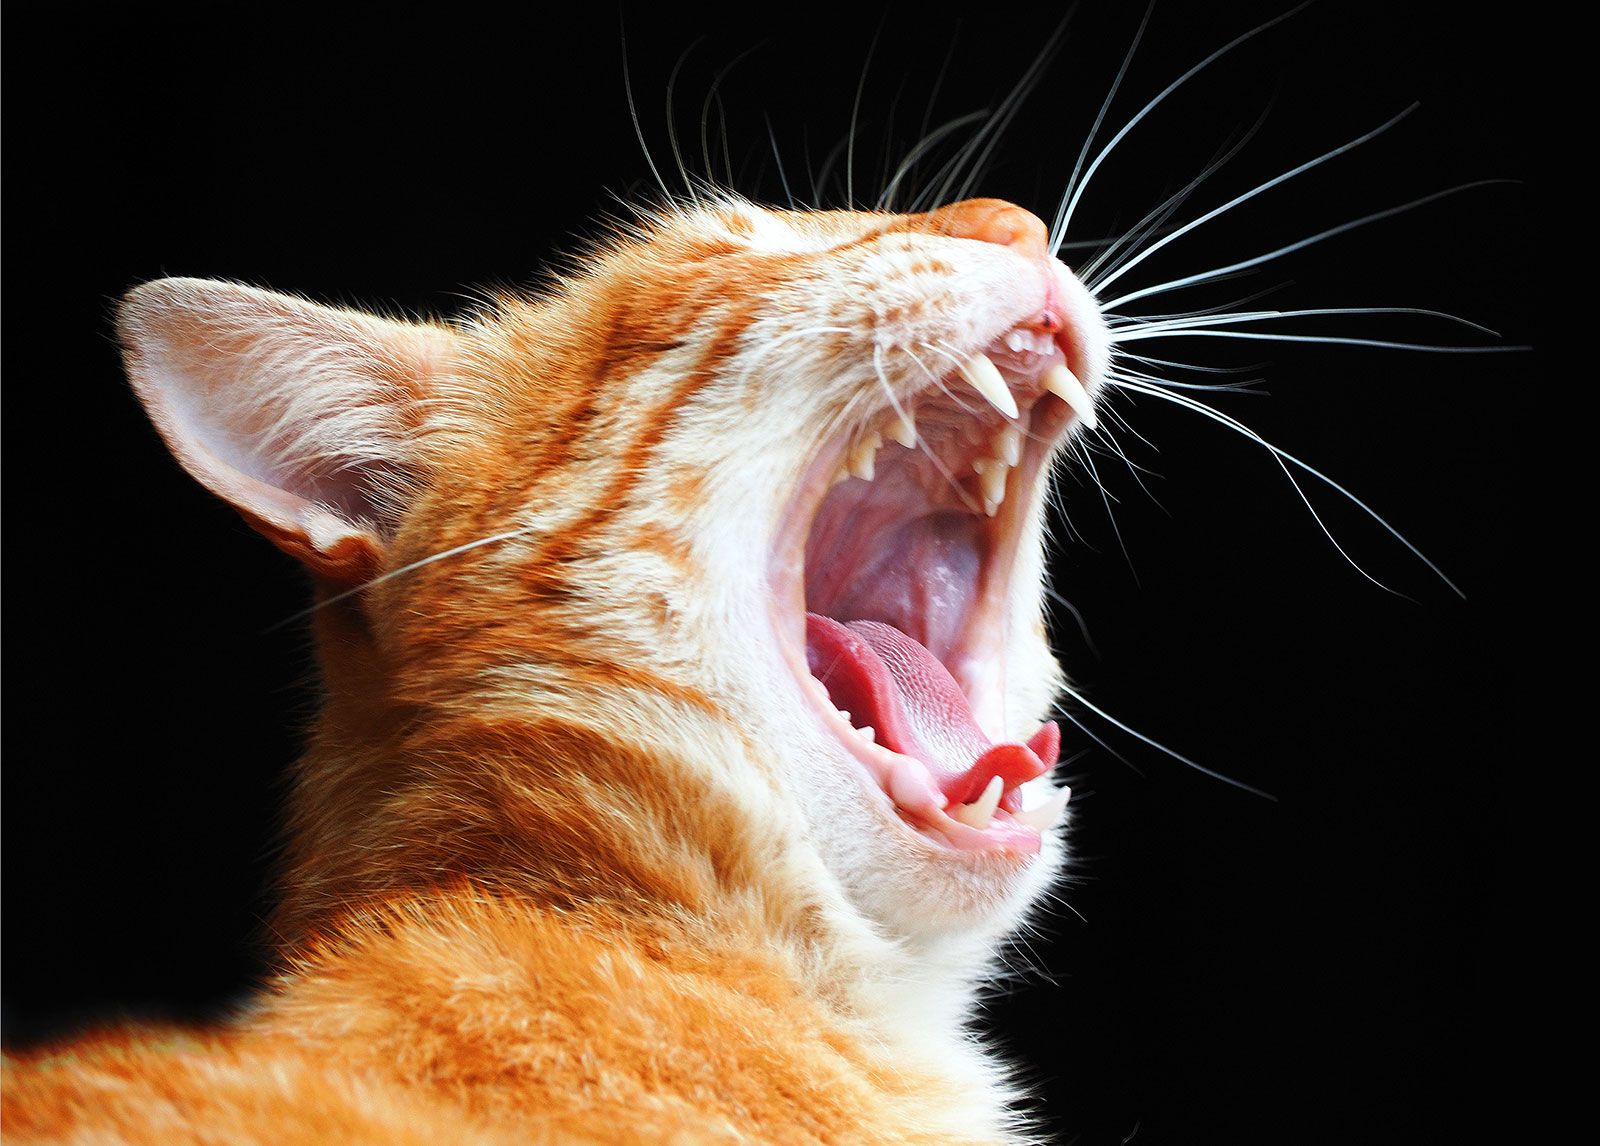
\includegraphics[width=.95\textwidth]{Orange-colored-cat-yawns-displaying-teeth} %{CS0031}
	\caption{Cat \cite{Cat}.}
	\label{fig:Cat}
	\end{figure}
	\section{Talk about the image}
	I have ask my mind to come up with a sentence to say about the cat.
	
	\printbibliography
	\addcontentsline{toc}{chapter}{Abbildungsverzeichnis}
	\listoffigures
	
\end{document}